\phantomsection
\addappheadtotoc
\chapter{Dev Manual}
\label{app:usermanual}
\section{Documentation}
All the documentation of the project is hosted by Github \cite{github} at \url{https://topodifogna.github.io/AdaptAnalyzer/}
\section{Build the Project}
The project has been set-up with the Gradle Build Tool \cite{gradle}; it is enough to execute the \texttt{createStandaloneJar} task defined in the main \texttt{build.gradle} file with the provided Gradle wrapper and it creates an executable Jar in the \texttt{distribution} subdirectory.
\section{Code Structure}
The tool has been developed in a modularized way, taking in consideration the MVC architectural pattern; to honor this pattern all the java classes are inside the \texttt{src\textbackslash java} folder and all the fxml file containing the view are inside the \texttt{src\textbackslash resources} folder.

\noindent The code is divided in four Java packages:
\begin{itemize}
	\item \texttt{generator}: contains the classes for the architecture generator.
	\item \texttt{gui}: contains all the classes that manage the view including all the controller for the fxml files.
	\item \texttt{metrics}: this package contains all the classes with the methods that allow to elaborate the data and return a result.
	\item \texttt{model}: contain the classes that represent the architecture and its elements; the class diagram is shown in Figure \ref{fig:aa-class}
\end{itemize}

\begin{figure}[ht]
	\centerline
	{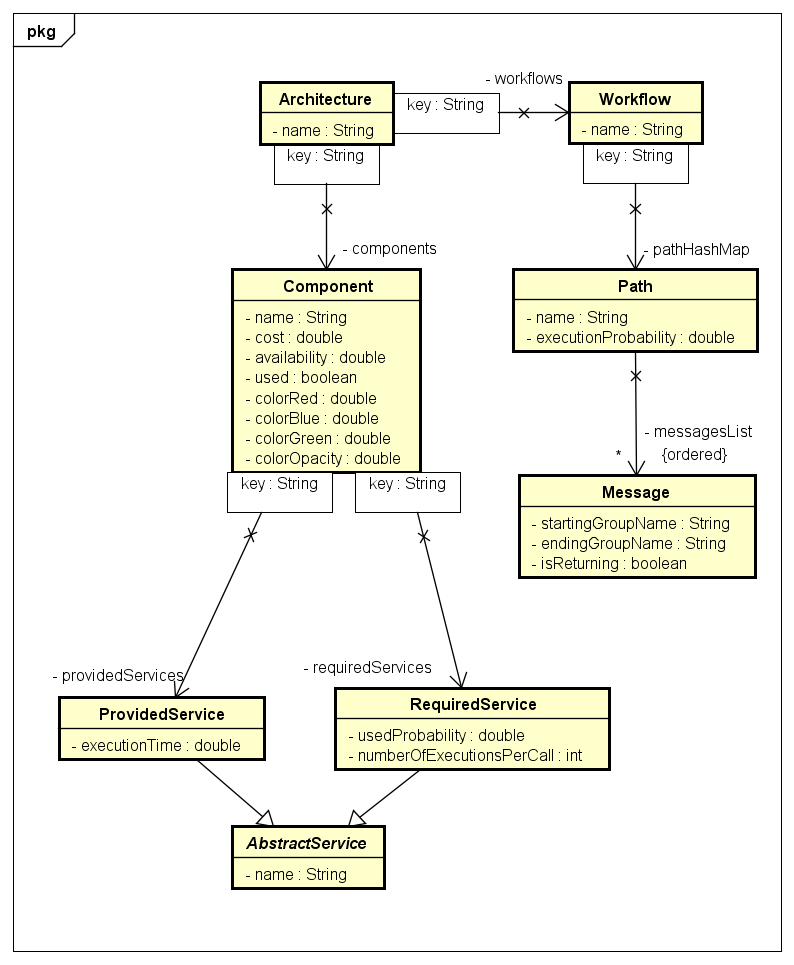
\includegraphics[scale=0.60]{img/adaptanalyzerclassdiag.png}}
	\caption[Adapt Analyzer Model Class Diagram]{Adapt Analyzer Model Class Diagram.}
	\label{fig:aa-class}
\end{figure}
